\documentclass{article}
\usepackage{nopageno}

\usepackage[margin=1.5cm]{geometry}


\usepackage{phoenician}

\usepackage{tikz}
\usetikzlibrary{decorations.pathmorphing}

\newcommand{\handdrawnhrule}{%
  \noindent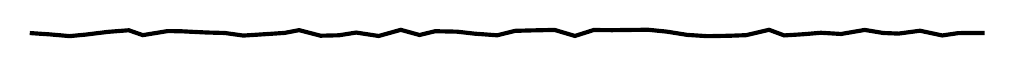
\begin{tikzpicture}
    \draw[line width=1.5pt, decorate, decoration={random steps, segment length=7pt, amplitude=1.2pt}] 
      (0,0) -- (\linewidth,0);
  \end{tikzpicture}%
}

\newcommand{\handline}{%
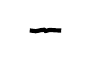
\begin{tikzpicture}[baseline=-0.5ex]
\draw[line width=1.5pt, decorate, decoration={random steps, amplitude=0.3pt, segment length=1pt}] 
  (0,0) -- (0.4,0);
\end{tikzpicture}%
}

\renewcommand{\labelitemi}{\handline}

\begin{document}
\phncfamily 

\noindent\textphnc{\LARGE{Boat Name Ephridia type Gaulos}}\newline\linebreak
\noindent\textphnc{\LARGE{Boat type Gaulos}}

\handdrawnhrule

\begin{itemize}
  \item \textphnc{\Large Cedar wood : two steres}
  \item \textphnc{\Large Pine wood : two steres}
  \item \textphnc{\Large Fine linen : twenty yards}
  \item \textphnc{\Large Tyrian purple dye : hundred Ounces}
  \item \textphnc{\Large Glassware : seventy eight pieces}
  \item \textphnc{\Large Metals (copper ten Kg, silver one Kg, iron hundred Kg, gold hundred g)}
  \item \textphnc{\Large Textiles : mixed hundred yards}
  \item \textphnc{\Large Wine : fifty clay jugs}
  \item \textphnc{\Large Salt : fifty Kg}
  \item \textphnc{\Large Horses : two stallions}
  \item \textphnc{\Large Ivory : twelve tusks and fragments}
  \item \textphnc{\Large Tortoise : twenty shells}
  \item \textphnc{\Large Spices (pepper fifty Kg, cinnamon twenty Kg, nard ten Kg)}
  \item \textphnc{\Large Slaves : two Lizardmen}
  \item \textphnc{\Large Sheep : four youngs}
  \item \textphnc{\Large Wool : five Ballots}
  \item \textphnc{\Large Perfumes: mixed five Litres}
  \item \textphnc{\Large Precious stones (fifteen emeralds, forty five agates)}
  \item \textphnc{\Large Metalwork (twenty two mixed crafted items)}
  \item \textphnc{\Large Olive oil : fifty clay jugs}
\end{itemize}

\newpage
\noindent\textphnc{\Large A\\ B\\ C\\ D\\ E\\ F\\ G\\ H\\ I\\ J\\ K\\ L\\ M\\ N\\ O\\ P\\ Q\\ R\\ S\\ T\\ U\\ V\\ W\\ X\\ Y\\ Z}


\end{document}
